\chapter{\ifenglish Introduction\else บทนำ\fi}

\section{\ifenglish Project rationale\else ที่มาของโครงงาน\fi}
\qquad ปัจจุบันการตรวจใบงานแบบกระดาษและการบันทึกคะแนนลงในคอมพิวเตอร์ยังคงใช้เวลาที่นานและมีความซ้ำซ้อน โดยกระบวนการนี้มีความซับซ้อนในหลายลำดับ ยกตัวอย่างเช่น อาจารย์ในมหาวิทยาลัยเชียงใหม่ที่สอนหลายกระบวนวิชามีปริมาณกระดาษข้อสอบและ ใบงานจำนวนมาก เมื่อมีการเปลี่ยนแปลงเกณฑ์การให้คะแนน จึงจำเป็นต้องกลับมาตรวจและคำนวณคะแนนใหม่อีกครั้ง ทำให้กระบวนการนี้เกิดความล่าช้าและการให้คะแนนในรูปแบบใบงานที่เป็นกระดาษยังซับซ้อน  ต้องบันทึกคะแนนลงในระบบคอมพิวเตอร์หรือ 
แพลตฟอร์มอื่นและนำไปวิเคราะห์สถิติในภายหลัง  การจัดเก็บใบงานในรูปแบบกระดาษต้องใช้พื้นที่ในการจัดเก็บที่มาก และการค้นหาใบงานจะยิ่งยากหากมีปริมาณใบงานมาก นอกจากนี้ยังเสี่ยงต่อการสูญหาย และหากนักศึกษายื่นขอตรวจคะแนนใหม่ จำเป็นต้องค้นหาใบงานเพื่อตรวจซ้ำอีกรอบ 

\qquad แพลตฟอร์มสำหรับการตรวจใบงานแบบกระดาษ (PaperGrader) เป็นแพลตฟอร์มที่เป็นทางเลือกสำหรับอาจารย์ในมหาวิทยาลัยเชียงใหม่ ที่จะเข้ามาช่วยในเรื่องการกำหนดเกณฑ์คะแนนที่ซับซ้อน การปรับเปลี่ยนเกณฑ์คะแนนระหว่างการตรวจ นอกจากนี้ยังช่วยให้นักศึกษาในมหาวิทยาลัยเชียงใหม่ สามารถติดตามคะแนนของใบงานและสามารถมีการยื่นคำร้องขอเพื่อขอรับการตรวจคะแนนใหม่จากอาจารย์ผู้สอน

\section{\ifenglish Objectives\else วัตถุประสงค์ของโครงงาน\fi}
    \begin{enumerate}
        \item เพื่อพัฒนาแพลตฟอร์มในการตรวจใบงานแบบกระดาษ  ที่จะเข้ามาช่วยลดความล่าช้าในการให้คะแนน และปรับเปลี่ยนเกณฑ์คะแนนในภายหลังของใบงาน
        \item เพื่อช่วยให้ผู้สอนสามารถวิเคราะห์สถิติคะแนน เพื่อใช้ในการปรับปรุงการออกข้อสอบ
        \item เพื่อช่วยให้นักศึกษาสามารถติดตามคะแนนของใบงานได้อย่างสะดวก และเห็นเกณฑ์การให้คะแนนอย่างชัดเจน
    \end{enumerate}

\section{\ifenglish Project scope\else ขอบเขตของโครงงาน\fi}

\subsection{\ifenglish Hardware scope\else ขอบเขตด้านฮาร์ดแวร์\fi}
\begin{enumerate}
    \item คอมพิวเตอร์หรือโน๊ตบุ๊คที่ใช้สำหรับระบบต้องสามารถเชื่อมต่อสัญญาณอินเทอร์เน็ต
\end{enumerate}

\subsection{\ifenglish Software scope\else ขอบเขตด้านซอฟต์แวร์\fi}
\begin{enumerate}
    \item  ผู้ใช้งานแพลตฟอร์มนี้ประกอบไปด้วย อาจารย์มหาวิทยาลัยเชียงใหม่ที่ต้องการตรวจใบงานแบบกระดาษ รวมถึงนักศึกษามหาวิทยาลัยเชียงใหม่ที่ต้องการติดตามคะแนนของใบงานและยื่นคำร้องขอเพื่อขอรับการตรวจคะแนนใหม่จากอาจารย์มหาวิทยาลัยเชียงใหม่ 
    \item การใช้งานในฟังก์ชันการอัปโหลดใบงาน จำเป็นต้องทำการอัปโหลดใบงานหรือข้อสอบเข้าสู่แพลตฟอร์ม เพื่อใช้งานแอปพลิเคชั่นในฟังก์ชั่นการใช้งานถัดๆ ไป 
    \item การกำหนด Bounding Box ของเทมเพลตในแต่ละข้อของใบงาน จะไม่สามารถกำหนด Bounding Box เกินหน้ากระดาษของข้อนั้นได้ 
\end{enumerate}

\section{\ifenglish Expected outcomes\else ประโยชน์ที่ได้รับ\fi}
    \subsection{อาจารย์มหาวิทยาลัยเชียงใหม่}
        \begin{enumerate}
            \renewcommand{\labelenumii}{\theenumi.\arabic{enumii}}
            \item ลดการจัดเตรียมพื้นที่ในการจัดเก็บเอกสาร
            \item ลดความล่าช้าในการคืนเอกสารหรือใบงาน เมื่อมีการใช้งาน
            \item ลดความผิดพลาดจากการปรับเปลี่ยนเกณฑ์คะแนน (Rubric)
            \item เพิ่มความสะดวกในการใช้แพลตฟอร์มในการตรวจคะแนนแบบออนไลน์
        \end{enumerate}

    \subsection{นักศึกษามหาวิทยาลัยเชียงใหม่}
        \begin{enumerate}
            \renewcommand{\labelenumii}{\theenumi.\arabic{enumii}}
            \item สามารถติดตามคะแนนของใบงานได้อย่างสะดวก
            \item เห็นเกณฑ์การให้คะแนนอย่างชัดเจน
        \end{enumerate}

    \subsection{กลุ่มวิจัยที่มีการนำข้อมูลไปใช้ต่อหรือไปใช้ร่วม}
        \begin{enumerate}
            \renewcommand{\labelenumii}{\theenumi.\arabic{enumii}}
            \item สามารถนำข้อมูลจากการติดไปใช้ต่อได้ โดยวิธีการส่งผ่าน API
        \end{enumerate}

\section{\ifenglish Technology and tools\else เทคโนโลยีและเครื่องมือที่ใช้\fi}
\subsection{Figma}
    \begin{figure}[ht]
        \centering
        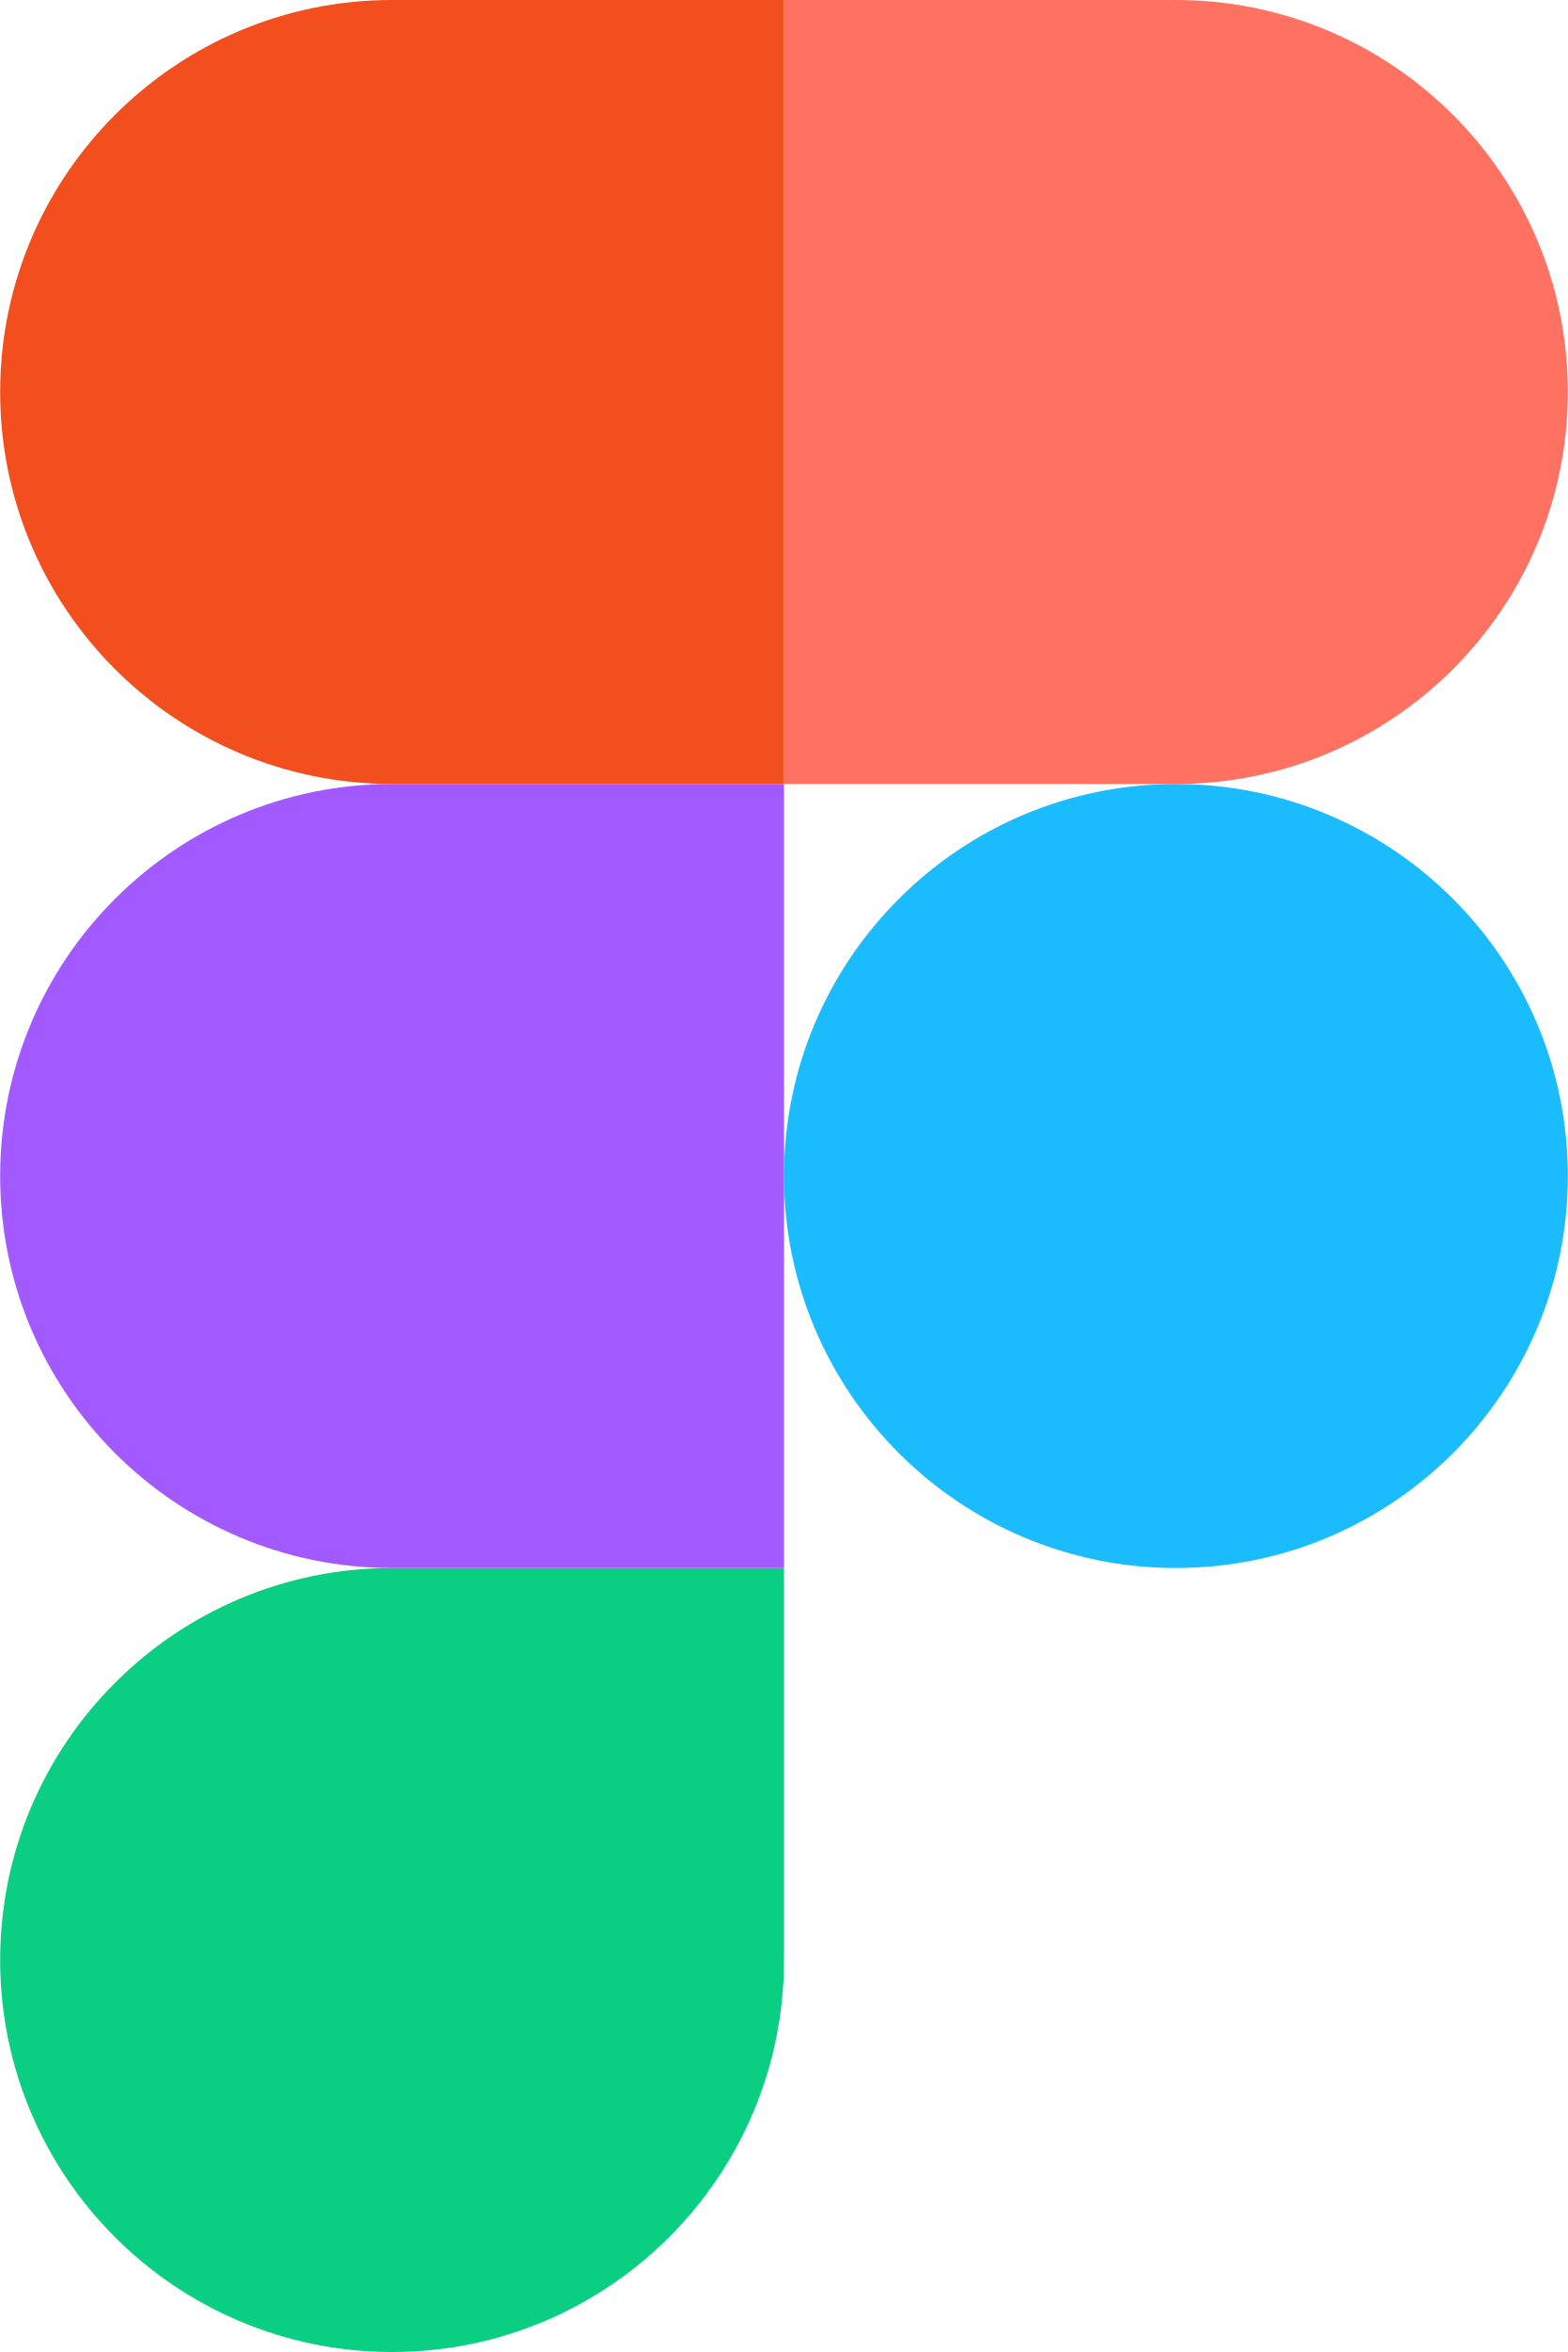
\includegraphics[width=0.2\textwidth, keepaspectratio]{image/Tools/figma-logo.png}
        \caption[Figma Logo]{Figma Logo\footnotemark}
        \label{fig:figma_logo}
        \footnotetext{\url{https://zemez.io/why-figma-is-used/?srsltid=AfmBOooK0t3pMnfb1b1HHTJDOZSJJD5aw_4zWWixCeSj-4oIL7x9e4HJ}/}
    \end{figure}
    \FloatBarrier
    \qquad Figma เป็นเครื่องมือที่ใช้ในการออกแบบ UI/UX ใช้งานผ่านเว็บ ทำให้สามารถทำงานร่วมกันได้ง่าย สามารถสร้าง Wireframe, Mockup, Prototype และ Design System ได้
\subsection{Next.js}
    \begin{figure}[ht]
        \centering
        
\includegraphics[width=0.35\textwidth]{image/Tools/nextjs-logo.png}
        \caption[Next.js Logo]{Next.js Logo\footnotemark}
        \label{fig:nextjs_logo}
        \footnotetext{\url{https://medium.com/geekculture/why-should-you-learn-next-js-in-2021-what-are-the-benefits-8292d79bc50c}}
    \end{figure}
    \FloatBarrier
    \qquad Next.js คือ เฟรมเวิร์ก (framework) ที่สร้างขึ้นบนพื้นฐานของ React.js ซึ่งเป็นไลบรารีสำหรับการพัฒนาเว็บแอปพลิเคชันที่ใช้ JavaScript โดย Next.js คุณสมบัติเด่นของ Next.js ได้แก่ การเรนเดอร์ฝั่งเซิร์ฟเวอร์ (server-side rendering) ที่ช่วยเพิ่มประสิทธิภาพในการโหลดหน้าเว็บ, การสร้างเส้นทางแบบไดนามิก (dynamic routing) ที่ช่วยให้สามารถจัดการเส้นทางของแอปพลิเคชันได้อย่างยืดหยุ่น, และการสนับสนุนการสร้างแอปพลิเคชันแบบสแตติก (static site generation) ที่ช่วยเพิ่มความเร็วในการโหลดหน้าเว็บ
    \subsubsection{ฟีเจอร์สำคัญของ Next.js}
    \begin{itemize}
        \item Server-side rendering (SSR): 
        \item Dynamic routing: 
        \item Hot reloading: 
    \end{itemize}
\subsection{Fiber}
    \begin{figure}[ht]
        \centering
        
\includegraphics[width=0.4\textwidth, keepaspectratio]{image/Tools/fiber-logo.png}
        \caption[Fiber Logo]{Fiber Logo\footnotemark}
        \label{fig:fiber_logo}
        \footnotetext{\url{https://medium.com/ieeeditu/fiber-5d58665f49ab}}
    \end{figure}
    \FloatBarrier
    \qquad Fiber คือ เว็บเฟรมเวิร์ก (framework) ที่พัฒนาขึ้นด้วยภาษา Go (Golang) ที่ได้แรงบันดาลใจมาจาก Express (node.js) ที่ build อยู่บน Fasthttp โดยมีเป้าหมายเพื่อให้การพัฒนาเว็บแอปพลิเคชันเป็นไปอย่างรวดเร็วและมีประสิทธิภาพ
    \subsubsection{ฟีเจอร์สำคัญของ Fiber}
    \begin{itemize}
        \item Routing management:
        \item Flexible middleware: 
        \item Rate Limiter:
        \item WebSocket support:
    \end{itemize}
\subsection{Docker}
    \begin{figure}[ht]
        \centering
        
\includegraphics[width=0.4\textwidth, keepaspectratio]{image/Tools/docker-logo.png}
        \caption[Docker Logo]{Docker Logo\footnotemark}
        \label{fig:docker_logo}
        \footnotetext{\url{https://www.docker.com/}}
    \end{figure}
    \FloatBarrier
    \qquad Docker คือ แพลตฟอร์มที่ช่วยให้นักพัฒนาสามารถสร้าง ทดสอบ และปรับใช้แอปพลิเคชันได้อย่างรวดเร็วผ่านการใช้คอนเทนเนอร์ (container) คอนเทนเนอร์เป็นสภาพแวดล้อมที่แยกจากกัน ซึ่งช่วยให้แอปพลิเคชันสามารถทำงานได้อย่างสม่ำเสมอในทุกสภาพแวดล้อม ไม่ว่าจะเป็นเครื่องพัฒนา เครื่องทดสอบ หรือเครื่องเซิร์ฟเวอร์จริง

\subsection{Virtual Machine}
    \begin{figure}[ht]
        \centering
        
\includegraphics[width=0.3\textwidth, keepaspectratio]{image/Tools/virtualbox-logo.png}
        \caption[Virtual Machine Logo]{Virtual Machine Logo\footnotemark}
        \label{fig:Virtual Machine_logo}
        \footnotetext{\url{https://www.vmware.com/topics/virtual-machine}}
    \end{figure}
    \FloatBarrier
    \qquad Virtual Machine (VM) คือ ซอฟต์แวร์ที่สร้างสภาพแวดล้อมเสมือนบนคอมพิวเตอร์จริง ซึ่งช่วยให้สามารถรันระบบปฏิบัติการและแอปพลิเคชันต่าง ๆ ได้อย่างแยกจากกัน VM ช่วยให้ผู้ใช้สามารถทดสอบซอฟต์แวร์ในสภาพแวดล้อมที่ปลอดภัย และสามารถจัดการทรัพยากรของระบบได้อย่างมีประสิทธิภาพ
\subsection{PostgreSQL}
    \begin{figure}[ht]
        \centering
        
\includegraphics[width=0.4\textwidth, keepaspectratio]{image/Tools/postgresql-logo.png}
        \caption[PostgreSQL Logo]{PostgreSQL Logo\footnotemark}
        \label{fig:postgresql_logo}
        \footnotetext{\url{https://www.postgresql.org/}}
    \end{figure}
    \FloatBarrier
\qquad PostgreSQL คือ ระบบฐานข้อมูลแบบ Relational Database Management System (RDBMS) ที่เป็นโอเพนซอร์ส มีความสามารถในการจัดการข้อมูลที่มีความซับซ้อน รวมถึงการจัดการข้อมูลที่มีความสัมพันธ์กัน

\subsection{MinIO}
    \begin{figure}[ht]
        \centering
        
\includegraphics[width=0.4\textwidth, keepaspectratio]{image/Tools/minio-logo.png}
        \caption[MinIO Logo]{MinIO Logo\footnotemark}
        \label{fig:minio_logo}
        \footnotetext{\url{https://medium.com/@dineshvarma.guduru/reading-and-writing-data-from-to-minio-using-spark-8371aefa96d2}}
    \end{figure}
    \FloatBarrier
\qquad MinIO คือ ระบบจัดเก็บข้อมูลแบบ Object Storage ที่มีความสามารถในการจัดการข้อมูลขนาดใหญ่และมีประสิทธิภาพสูง โดย MinIO ถูกออกแบบมาเพื่อรองรับการใช้งานในสภาพแวดล้อมที่ต้องการความเร็วและความน่าเชื่อถือสูง เช่น การจัดเก็บข้อมูลสำหรับแอปพลิเคชันที่ต้องการประสิทธิภาพสูง หรือการจัดเก็บข้อมูลในระบบคลาวด์

\section{\ifenglish Project plan\else แผนการดำเนินงาน\fi}

\begin{plan}{6}{2024}{10}{2025}
    \planitem{6}{2024}{6}{2024}{เลือกหัวข้อโครงการ}
    \planitem{6}{2024}{6}{2024}{เลือกอาจารย์ที่ปรึกษา}
    \planitem{6}{2024}{7}{2024}{สํารวจความต้องการของผู้ใช้}
    \planitem{6}{2024}{8}{2024}{ศึกษาระบบ}
\end{plan}

\begin{plan}{6}{2024}{10}{2025}
    \planitem{6}{2024}{10}{2024}{ออกแบบ UX/ UI และ feature ต่างๆ}
    \planitem{10}{2024}{10}{2025}{พัฒนา Frontend}
    \planitem{10}{2024}{10}{2025}{พัฒนา Backend}
    \planitem{10}{2024}{4}{2025}{ออกแบบฐานข้อมูล}
\end{plan}


\section{\ifenglish Roles and responsibilities\else บทบาทและความรับผิดชอบ\fi}
    \begin{itemize}
        \item นายคณพัฒน์ ประเพชร รับผิดชอบในการ ทําหน้าที่ในการออกแบบและพัฒนาส่วน
ติดต่อผู้ใช้ (Frontend Development) โดยรับผิดชอบออกแบบหน้าเว็บแอปพลิเคชัน ประสบการณ์
ผู้ใช้ และการพัฒนาฟังก์ชันต่างๆ
        \item นายจิรายุ จิตรเปรม รับผิดชอบในการ
        \item นายวิศรุต สาดา รับผิดชอบในการ
    \end{itemize}

\section{\ifenglish%
Impacts of this project on society, health, safety, legal, and cultural issues
\else%
ผลกระทบด้านสังคม สุขภาพ ความปลอดภัย กฎหมาย และวัฒนธรรม
\fi}
\qquad แพลตฟอร์มนี้จะสามารถช่วยให้ผู้งานมีความสะดวกในการตรวจใบงานแบบกระดาษ และมีทางเลือกในการใช้แพลตฟอร์มสําหรับการตรวจใบงานแบบกระดาษมากยิ่งขึ้น